\begin{figure}
    % WARNING: DO NOT CHANGE MANUALLY, CHANGES WILL BE OVERWRITTEN
    \centering
    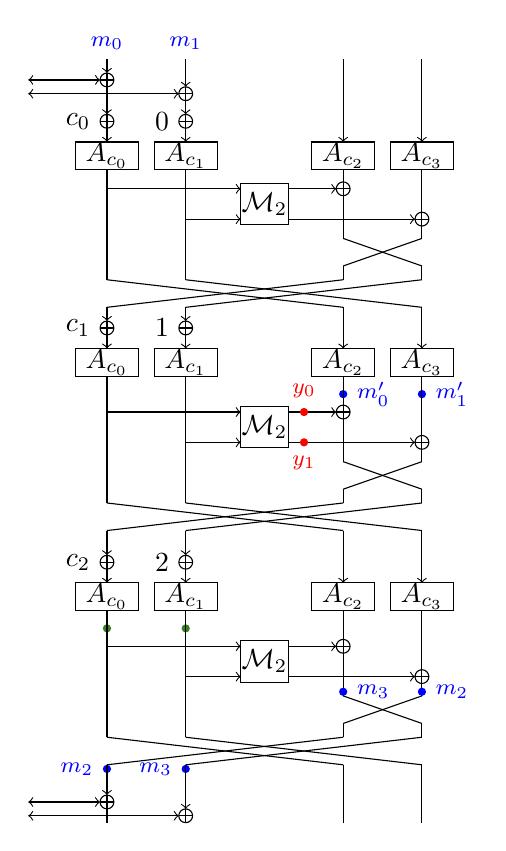
\begin{tikzpicture}[xscale=1.0,yscale=-0.7]
        \draw (-2.0,0.0) node[anchor=south] {\footnotesize\color{blue}$m_0$};
        \draw (-1.0,0.0) node[anchor=south] {\footnotesize\color{blue}$m_1$};
        \draw[->] (-2.0,0.0) -- (-2.0,0.25);
        \draw (-2.0,0.375) ellipse (0.0875 and 0.125);
        \draw (-2.0,0.25) -- (-2.0,0.5);
        \draw (-2.0875,0.375) -- (-1.9125,0.375);
        \draw (-2.0,0.5) -- (-2.0,0.75);
        \draw[<->] (-3.0,0.375) -- (-2.0875,0.375);
        \draw[->] (-1.0,0.0) -- (-1.0,0.5);
        \draw (-1.0,0.625) ellipse (0.0875 and 0.125);
        \draw (-1.0,0.5) -- (-1.0,0.75);
        \draw (-1.0875,0.625) -- (-0.9125,0.625);
        \draw (-1.0,0.75) -- (-1.0,0.75);
        \draw[<->] (-3.0,0.625) -- (-1.0875,0.625);
        \draw (1.0,0.0) -- (1.0,0.75);
        \draw (2.0,0.0) -- (2.0,0.75);
        \draw[->] (-2.0,0.75) -- (-2.0,1.0);
        \draw (-2.0,1.125) ellipse (0.0875 and 0.125);
        \draw (-2.0,1.0) -- (-2.0,1.25);
        \draw (-2.0875,1.125) -- (-1.9125,1.125);
        \draw (-2.0875,1.125) node[anchor=east] {$c_0$};
        \draw[->] (-2.0,1.25) -- (-2.0,1.5);
        \draw (-2.4,1.5) rectangle (-1.6,2.0) node[pos=0.5] {$A_{c_0}$};
        \draw (-2.0,2.0) -- (-2.0,2.25);
        \draw[->] (-1.0,0.75) -- (-1.0,1.0);
        \draw (-1.0,1.125) ellipse (0.0875 and 0.125);
        \draw (-1.0,1.0) -- (-1.0,1.25);
        \draw (-1.0875,1.125) -- (-0.9125,1.125);
        \draw (-1.0875,1.125) node[anchor=east] {$0$};
        \draw[->] (-1.0,1.25) -- (-1.0,1.5);
        \draw (-1.4,1.5) rectangle (-0.6,2.0) node[pos=0.5] {$A_{c_1}$};
        \draw (-1.0,2.0) -- (-1.0,2.25);
        \draw[->] (1.0,0.75) -- (1.0,1.5);
        \draw (0.6,1.5) rectangle (1.4,2.0) node[pos=0.5] {$A_{c_2}$};
        \draw (1.0,2.0) -- (1.0,2.25);
        \draw[->] (2.0,0.75) -- (2.0,1.5);
        \draw (1.6,1.5) rectangle (2.4,2.0) node[pos=0.5] {$A_{c_3}$};
        \draw (2.0,2.0) -- (2.0,2.25);
        \draw (-0.3,2.25) rectangle (0.3,3.0) node[pos=0.5] {$\mathcal{M}_{2}$};
        \draw[->] (-2.0,2.35) -- (-0.3,2.35);
        \draw (1.0,2.35) ellipse (0.0875 and 0.125);
        \draw (1.0,2.225) -- (1.0,2.475);
        \draw (0.9125,2.35) -- (1.0875,2.35);
        \draw[->] (0.3,2.35) -- (0.9125,2.35);
        \draw[->] (-1.0,2.9) -- (-0.3,2.9);
        \draw (2.0,2.9) ellipse (0.0875 and 0.125);
        \draw (2.0,2.775) -- (2.0,3.025);
        \draw (1.9125,2.9) -- (2.0875,2.9);
        \draw[->] (0.3,2.9) -- (1.9125,2.9);
        \draw (-2.0,2.25) -- (-2.0,3.25);
        \draw (-1.0,2.25) -- (-1.0,3.25);
        \draw (1.0,2.25) -- (1.0,3.25);
        \draw (2.0,2.25) -- (2.0,3.25);
        \draw (-2.0,3.25) -- (-2.0,4.0);
        \draw (-1.0,3.25) -- (-1.0,4.0);
        \draw (2.0,3.25) -- (1.0,3.75);
        \draw (1.0,3.25) -- (2.0,3.75);
        \draw (1.0,3.75) -- (1.0,4.0);
        \draw (2.0,3.75) -- (2.0,4.0);
        \draw (-2.0,4.0) -- (1.0,4.5);
        \draw (-1.0,4.0) -- (2.0,4.5);
        \draw (1.0,4.0) -- (-2.0,4.5);
        \draw (2.0,4.0) -- (-1.0,4.5);
        \draw[->] (-2.0,4.5) -- (-2.0,4.75);
        \draw (-2.0,4.875) ellipse (0.0875 and 0.125);
        \draw (-2.0,4.75) -- (-2.0,5.0);
        \draw (-2.0875,4.875) -- (-1.9125,4.875);
        \draw (-2.0875,4.875) node[anchor=east] {$c_1$};
        \draw[->] (-2.0,5.0) -- (-2.0,5.25);
        \draw (-2.4,5.25) rectangle (-1.6,5.75) node[pos=0.5] {$A_{c_0}$};
        \draw (-2.0,5.75) -- (-2.0,6.0);
        \draw[->] (-1.0,4.5) -- (-1.0,4.75);
        \draw (-1.0,4.875) ellipse (0.0875 and 0.125);
        \draw (-1.0,4.75) -- (-1.0,5.0);
        \draw (-1.0875,4.875) -- (-0.9125,4.875);
        \draw (-1.0875,4.875) node[anchor=east] {$1$};
        \draw[->] (-1.0,5.0) -- (-1.0,5.25);
        \draw (-1.4,5.25) rectangle (-0.6,5.75) node[pos=0.5] {$A_{c_1}$};
        \draw (-1.0,5.75) -- (-1.0,6.0);
        \draw[->] (1.0,4.5) -- (1.0,5.25);
        \draw (0.6,5.25) rectangle (1.4,5.75) node[pos=0.5] {$A_{c_2}$};
        \draw (1.0,5.75) -- (1.0,6.0);
        \draw[->] (2.0,4.5) -- (2.0,5.25);
        \draw (1.6,5.25) rectangle (2.4,5.75) node[pos=0.5] {$A_{c_3}$};
        \draw (2.0,5.75) -- (2.0,6.0);
        \fill[blue] (1.0,6.075) ellipse (0.0525 and 0.075);
        \draw (1.0525,6.075) node[anchor=west] {\footnotesize\color{blue}$m_0'$};
        \fill[blue] (2.0,6.075) ellipse (0.0525 and 0.075);
        \draw (2.0525,6.075) node[anchor=west] {\footnotesize\color{blue}$m_1'$};
        \draw (-2.0,6.0) -- (-2.0,6.3);
        \draw (-1.0,6.0) -- (-1.0,6.3);
        \draw (1.0,6.0) -- (1.0,6.3);
        \draw (2.0,6.0) -- (2.0,6.3);
        \draw (-0.3,6.3) rectangle (0.3,7.05) node[pos=0.5] {$\mathcal{M}_{2}$};
        \draw[->] (-2.0,6.4) -- (-0.3,6.4);
        \draw (1.0,6.4) ellipse (0.0875 and 0.125);
        \draw (1.0,6.275) -- (1.0,6.525);
        \draw (0.9125,6.4) -- (1.0875,6.4);
        \draw[->] (0.3,6.4) -- (0.9125,6.4);
        \fill[red] (0.5025,6.4) ellipse (0.0525 and 0.075);
        \draw (0.5025,6.325) node[anchor=south] {\footnotesize\color{red}$y_0$};
        \draw[->] (-1.0,6.95) -- (-0.3,6.95);
        \draw (2.0,6.95) ellipse (0.0875 and 0.125);
        \draw (2.0,6.825) -- (2.0,7.075);
        \draw (1.9125,6.95) -- (2.0875,6.95);
        \draw[->] (0.3,6.95) -- (1.9125,6.95);
        \fill[red] (0.5025,6.95) ellipse (0.0525 and 0.075);
        \draw (0.5025,7.025) node[anchor=north] {\footnotesize\color{red}$y_1$};
        \draw (-2.0,6.3) -- (-2.0,7.3);
        \draw (-1.0,6.3) -- (-1.0,7.3);
        \draw (1.0,6.3) -- (1.0,7.3);
        \draw (2.0,6.3) -- (2.0,7.3);
        \draw (-2.0,7.3) -- (-2.0,8.05);
        \draw (-1.0,7.3) -- (-1.0,8.05);
        \draw (2.0,7.3) -- (1.0,7.8);
        \draw (1.0,7.3) -- (2.0,7.8);
        \draw (1.0,7.8) -- (1.0,8.05);
        \draw (2.0,7.8) -- (2.0,8.05);
        \draw (-2.0,8.05) -- (1.0,8.55);
        \draw (-1.0,8.05) -- (2.0,8.55);
        \draw (1.0,8.05) -- (-2.0,8.55);
        \draw (2.0,8.05) -- (-1.0,8.55);
        \draw (-2.0,8.55) -- (-2.0,8.65);
        \draw (-1.0,8.55) -- (-1.0,8.65);
        \draw (1.0,8.55) -- (1.0,8.65);
        \draw (2.0,8.55) -- (2.0,8.65);
        \draw (-2.0,8.65) -- (-2.0,8.75);
        \draw (-1.0,8.65) -- (-1.0,8.75);
        \draw (1.0,8.65) -- (1.0,8.75);
        \draw (2.0,8.65) -- (2.0,8.75);
        \draw[->] (-2.0,8.75) -- (-2.0,9.0);
        \draw (-2.0,9.125) ellipse (0.0875 and 0.125);
        \draw (-2.0,9.0) -- (-2.0,9.25);
        \draw (-2.0875,9.125) -- (-1.9125,9.125);
        \draw (-2.0875,9.125) node[anchor=east] {$c_2$};
        \draw[->] (-2.0,9.25) -- (-2.0,9.5);
        \draw (-2.4,9.5) rectangle (-1.6,10.0) node[pos=0.5] {$A_{c_0}$};
        \draw (-2.0,10.0) -- (-2.0,10.25);
        \draw[->] (-1.0,8.75) -- (-1.0,9.0);
        \draw (-1.0,9.125) ellipse (0.0875 and 0.125);
        \draw (-1.0,9.0) -- (-1.0,9.25);
        \draw (-1.0875,9.125) -- (-0.9125,9.125);
        \draw (-1.0875,9.125) node[anchor=east] {$2$};
        \draw[->] (-1.0,9.25) -- (-1.0,9.5);
        \draw (-1.4,9.5) rectangle (-0.6,10.0) node[pos=0.5] {$A_{c_1}$};
        \draw (-1.0,10.0) -- (-1.0,10.25);
        \draw[->] (1.0,8.75) -- (1.0,9.5);
        \draw (0.6,9.5) rectangle (1.4,10.0) node[pos=0.5] {$A_{c_2}$};
        \draw (1.0,10.0) -- (1.0,10.25);
        \draw[->] (2.0,8.75) -- (2.0,9.5);
        \draw (1.6,9.5) rectangle (2.4,10.0) node[pos=0.5] {$A_{c_3}$};
        \draw (2.0,10.0) -- (2.0,10.25);
        \fill[OliveGreen] (-2.0,10.325) ellipse (0.0525 and 0.075);
        \fill[OliveGreen] (-1.0,10.325) ellipse (0.0525 and 0.075);
        \draw (-2.0,10.25) -- (-2.0,10.55);
        \draw (-1.0,10.25) -- (-1.0,10.55);
        \draw (1.0,10.25) -- (1.0,10.55);
        \draw (2.0,10.25) -- (2.0,10.55);
        \draw (-0.3,10.55) rectangle (0.3,11.3) node[pos=0.5] {$\mathcal{M}_{2}$};
        \draw[->] (-2.0,10.65) -- (-0.3,10.65);
        \draw (1.0,10.65) ellipse (0.0875 and 0.125);
        \draw (1.0,10.525) -- (1.0,10.775);
        \draw (0.9125,10.65) -- (1.0875,10.65);
        \draw[->] (0.3,10.65) -- (0.9125,10.65);
        \draw[->] (-1.0,11.2) -- (-0.3,11.2);
        \draw (2.0,11.2) ellipse (0.0875 and 0.125);
        \draw (2.0,11.075) -- (2.0,11.325);
        \draw (1.9125,11.2) -- (2.0875,11.2);
        \draw[->] (0.3,11.2) -- (1.9125,11.2);
        \draw (-2.0,10.55) -- (-2.0,11.55);
        \draw (-1.0,10.55) -- (-1.0,11.55);
        \draw (1.0,10.55) -- (1.0,11.55);
        \draw (2.0,10.55) -- (2.0,11.55);
        \fill[blue] (1.0,11.475) ellipse (0.0525 and 0.075);
        \draw (1.0525,11.475) node[anchor=west] {\footnotesize\color{blue}$m_3$};
        \fill[blue] (2.0,11.475) ellipse (0.0525 and 0.075);
        \draw (2.0525,11.475) node[anchor=west] {\footnotesize\color{blue}$m_2$};
        \draw (-2.0,11.55) -- (-2.0,12.3);
        \draw (-1.0,11.55) -- (-1.0,12.3);
        \draw (2.0,11.55) -- (1.0,12.05);
        \draw (1.0,11.55) -- (2.0,12.05);
        \draw (1.0,12.05) -- (1.0,12.3);
        \draw (2.0,12.05) -- (2.0,12.3);
        \draw (-2.0,12.3) -- (1.0,12.8);
        \draw (-1.0,12.3) -- (2.0,12.8);
        \draw (1.0,12.3) -- (-2.0,12.8);
        \draw (2.0,12.3) -- (-1.0,12.8);
        \fill[blue] (-2.0,12.875) ellipse (0.0525 and 0.075);
        \draw (-2.0525,12.875) node[anchor=east] {\footnotesize\color{blue}$m_2$};
        \fill[blue] (-1.0,12.875) ellipse (0.0525 and 0.075);
        \draw (-1.0525,12.875) node[anchor=east] {\footnotesize\color{blue}$m_3$};
        \draw (-2.0,12.8) -- (-2.0,13.1);
        \draw (-1.0,12.8) -- (-1.0,13.1);
        \draw (1.0,12.8) -- (1.0,13.1);
        \draw (2.0,12.8) -- (2.0,13.1);
        \draw[->] (-2.0,13.1) -- (-2.0,13.35);
        \draw (-2.0,13.475) ellipse (0.0875 and 0.125);
        \draw (-2.0,13.35) -- (-2.0,13.6);
        \draw (-2.0875,13.475) -- (-1.9125,13.475);
        \draw (-2.0,13.6) -- (-2.0,13.85);
        \draw[<->] (-3.0,13.475) -- (-2.0875,13.475);
        \draw[->] (-1.0,13.1) -- (-1.0,13.6);
        \draw (-1.0,13.725) ellipse (0.0875 and 0.125);
        \draw (-1.0,13.6) -- (-1.0,13.85);
        \draw (-1.0875,13.725) -- (-0.9125,13.725);
        \draw (-1.0,13.85) -- (-1.0,13.85);
        \draw[<->] (-3.0,13.725) -- (-1.0875,13.725);
        \draw (1.0,13.1) -- (1.0,13.85);
        \draw (2.0,13.1) -- (2.0,13.85);
    \end{tikzpicture}
    \caption{Analysis of 3-step Schwaemm128-128.}
    \label{fig:mitm3}
\end{figure}
